% Pregunta 3 - Ayudantía 8

\textbf{P3)} \textcolor{red}{[Prueba 3 - 2025-10]} Una cuerda está vibrando con $f=5\ \mathrm{Hz}$ y amplitud $A$ sobre un plano vertical, de modo que genera una onda transversal que se mueve hacia la derecha con velocidad $v$, tal como muestra la figura. La función de onda puede considerarse como $y(x,t)=A\cos(kx-\omega t)$, donde $k$ es el número de onda y $\omega$ la frecuencia angular. $k=2\pi/\lambda$ y $\omega=2\pi f$. Use dos decimales.

\begin{center}
	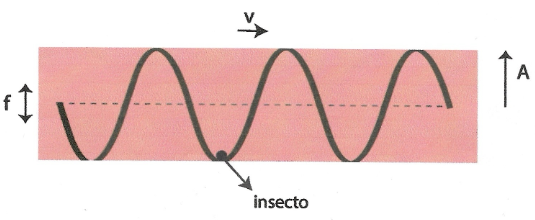
\includegraphics[width=0.6\textwidth]{../imagenes/imagen p3 a8.PNG}
\end{center}

Un insecto de masa $m$ está durmiendo pegado a la parte superior de la cuerda. Determine la amplitud $A$ (en cm) necesaria para que cuando la onda vibre en la posición del insecto y éste esté en la altura más baja (ver figura) sienta una fuerza $5G$. Cuando estamos en la situación estándar sentimos $1G$. Si estamos acelerados $g$ hacia arriba sentimos $2G$, si estamos acelerados $2g$ hacia arriba sentimos $3G$, etc.

% Respuesta / espacio para soluciones

